\documentclass[11pt,oneside]{article}

\usepackage[a4paper,margin=27mm,headheight=15pt]{geometry}
\usepackage[T1]{fontenc}
\usepackage[utf8]{inputenc}
\IfFileExists{libertinus.sty}{\usepackage{libertinus}}{\usepackage{lmodern}}
\usepackage{microtype}
\usepackage{amsmath,amssymb,amsthm,mathtools,mathrsfs}
\usepackage{bm}
\usepackage{booktabs,longtable,array,tabularx}
\usepackage{graphicx}
\usepackage{pgfplots}
\usepackage{xcolor}
\usepackage{enumitem}
\usepackage{fancyhdr}
\usepackage{titlesec}
\usepackage{listings}
\usepackage{xurl}
\usepackage{hyperref}
\usepackage[nameinlink,noabbrev]{cleveref}

\definecolor{linkblue}{RGB}{25,75,135}
\definecolor{shadegray}{RGB}{246,247,249}
\definecolor{rulegray}{RGB}{195,201,208}
\definecolor{codegreen}{RGB}{40,105,72}
\definecolor{codepurple}{RGB}{105,55,125}
\pgfplotsset{compat=1.18}
\hypersetup{
  colorlinks=true,
  linkcolor=linkblue,
  citecolor=linkblue,
  urlcolor=linkblue,
  pdftitle={Repeated Integration and Rvachev's Up-Function},
  pdfauthor={Complementary report for Vladimir Reshetnikov's ProveIt repository}
}

\pagestyle{fancy}
\fancyhf{}
\fancyhead[L]{\small Repeated integration and Rvachev's up-function}
\fancyhead[R]{\small\nouppercase{\leftmark}}
\fancyfoot[C]{\thepage}
\renewcommand{\headrulewidth}{0.4pt}

\titleformat{\section}{\Large\bfseries}{\thesection}{0.7em}{}
\titleformat{\subsection}{\large\bfseries}{\thesubsection}{0.7em}{}
\titleformat{\subsubsection}{\normalsize\bfseries}{\thesubsubsection}{0.7em}{}

\setcounter{secnumdepth}{3}
\setcounter{tocdepth}{2}
\setlist[itemize]{leftmargin=2em,itemsep=0.25em,topsep=0.4em}
\setlist[enumerate]{leftmargin=2.3em,itemsep=0.25em,topsep=0.4em}
\setlength{\emergencystretch}{2em}

\newtheorem{theorem}{Theorem}[section]
\newtheorem{proposition}[theorem]{Proposition}
\newtheorem{lemma}[theorem]{Lemma}
\newtheorem{corollary}[theorem]{Corollary}
\theoremstyle{definition}
\newtheorem{definition}[theorem]{Definition}
\newtheorem{example}[theorem]{Example}
\theoremstyle{remark}
\newtheorem{remark}[theorem]{Remark}
\newtheorem{warning}[theorem]{Warning}

\newcommand{\R}{\mathbb R}
\newcommand{\N}{\mathbb N}
\newcommand{\E}{\mathbb E}
\newcommand{\Prob}{\mathbb P}
\newcommand{\Var}{\operatorname{Var}}
\newcommand{\Law}{\mathcal L}
\newcommand{\Up}{\operatorname{up}}
\newcommand{\sinc}{\operatorname{sinc}}
\newcommand{\supp}{\operatorname{supp}}
\newcommand{\conv}{*}
\newcommand{\ind}{\mathbf 1}
\newcommand{\wt}{\operatorname{wt}}
\newcommand{\dd}{\,\mathrm d}
\newcommand{\norm}[1]{\left\lVert#1\right\rVert}
\newcommand{\abs}[1]{\left\lvert#1\right\rvert}
\newcommand{\pos}[1]{\left(#1\right)_{+}}
\newcommand{\floor}[1]{\left\lfloor#1\right\rfloor}
\newcommand{\ceil}[1]{\left\lceil#1\right\rceil}
\newcommand{\Binom}[2]{\binom{#1}{#2}}
\newcommand{\e}{\mathrm e}
\newcommand{\iu}{\mathrm i}
\newcommand{\D}{\mathrm D}

\newenvironment{proofidea}{\par\noindent\textit{Proof idea.}\ }{\hfill$\square$\par}
\newenvironment{boxedremark}{%
  \par\smallskip\noindent\begin{center}\begin{minipage}{0.94\textwidth}%
  \color{black}\hrule\vspace{0.6em}\small
}{%
  \vspace{0.6em}\hrule\end{minipage}\end{center}\smallskip
}

\lstdefinestyle{reportcode}{
  backgroundcolor=\color{shadegray},
  basicstyle=\ttfamily\small,
  keywordstyle=\color{linkblue}\bfseries,
  commentstyle=\color{codegreen},
  stringstyle=\color{codepurple},
  numbers=left,
  numberstyle=\tiny\color{gray},
  numbersep=8pt,
  frame=single,
  rulecolor=\color{rulegray},
  breaklines=true,
  showstringspaces=false,
  tabsize=4,
  columns=fullflexible
}

\title{\textbf{Repeated Integration and Rvachev's Up-Function}\\[0.45em]
\large Exact finite splines, Thue--Morse structure, and sharp convergence}
\author{Complementary report to \emph{The Fabius Function and Rvachev's Up-Function}\\
Vladimir Reshetnikov's \texttt{ProveIt} repository}
\date{25 August 2026}

\begin{document}
\maketitle

\begin{abstract}
A Math Stack Exchange question asks for a closed form for the sequence
\[
 f_0(x)=\frac12\ind_{(-1,1)}(x),\qquad
 f_n(x)=2\int_{-1}^{x}\bigl(f_{n-1}(2t+1)-f_{n-1}(2t-1)\bigr)\dd t.
\]
The first integration produces the piecewise linear tent
$f_1(x)=\pos{1-|x|}$, and the subsequent iterates visually converge very rapidly to
Rvachev's compactly supported $C^\infty$ up-function.  This report gives a complete
finite-stage description and a sharp convergence theorem.

The integral operator is exactly a probabilistic averaging operator: if $g$ is the density
of $Y$ and $U$ is uniform on $[-1,1]$, then the next density is that of $(Y+U)/2$.
Consequently, for $n\ge1$,
\[
 f_n=u_{2^{-1}}\conv u_{2^{-2}}\conv\cdots\conv u_{2^{-n}}\conv u_{2^{-n}},
 \qquad
 u_a(x)=\frac1{2a}\ind_{[-a,a]}(x).
\]
This identifies $f_n$ as a nonuniform box spline.  Collapsing its general
inclusion--exclusion formula with the Thue--Morse generating polynomial yields, for
$n\ge1$,
\[
 f_n(x)=\frac{2^{n(n+1)/2-1}}{n!}
 \sum_{j=0}^{2^n}\bigl(\tau_n(j)-\tau_n(j-1)\bigr)
 \pos{x+1-\frac{j}{2^{n-1}}}^{n},
\]
where $\tau_n(j)=(-1)^{\wt(j)}$ on $0\le j<2^n$ and is zero outside that range.
The $n$th derivative is therefore a rescaled Thue--Morse step function.

The principal quantitative result derived here is exact, rather than merely asymptotic.  For every
fixed $r\ge0$ and every $n\ge r+2$,
\[
 \boxed{\displaystyle
 \norm{f_n^{(r)}-\Up^{(r)}}_\infty
 =\frac{2^{\binom{r+3}{2}}}{9\,4^n}.}
\]
Thus, once the $r$th derivative has passed its first admissible spline stage, every further
integration divides its uniform error by exactly four.  In the indexing that starts with the
piecewise linear tent $g_0=f_1$, this becomes
\[
 \norm{g_m-\Up}_\infty=\frac{2}{9\,4^m}\qquad(m\ge1),
\]
while the exceptional initial error is $\norm{g_0-\Up}_\infty=13/72$.
The proof is based on an exact Peano-kernel identity.  The comparison kernel between a
uniform random variable and the up-distributed random variable has both integral and
maximum equal to $1/9$; the finite partial density has disjoint extremal plateaux whose
height is known exactly.  Their combination gives both the upper bound and matching
extremizers.
\end{abstract}

\tableofcontents
\newpage

\section{The problem, the indexing, and the answer}
\label{sec:introduction}

The recurrence considered in the Math Stack Exchange question
\cite{mse-question,mse-answer} is
\begin{equation}
 f_0(x)=\frac12\ind_{(-1,1)}(x),
 \qquad
 f_n(x)=2\int_{-1}^{x}
 \bigl(f_{n-1}(2t+1)-f_{n-1}(2t-1)\bigr)\dd t.
 \label{eq:original-recurrence}
\end{equation}
Changing the values of $f_0$ at $x=\pm1$ changes neither any later iterate nor any of the
norm statements below.  We therefore use whichever endpoint convention is convenient.

There is a small indexing issue in the informal description of the construction.  The
literal seed $f_0$ in \eqref{eq:original-recurrence} is piecewise constant; the first iterate
is the piecewise linear function
\begin{equation}
 f_1(x)=\pos{1-|x|}.
 \label{eq:tent}
\end{equation}
When one says that the up-function arises by ``repeatedly integrating a piecewise linear
function,'' the natural indexing is therefore
\begin{equation}
 g_m=f_{m+1},\qquad g_0(x)=\pos{1-|x|}.
 \label{eq:linear-indexing}
\end{equation}
Both indexings will be retained: $f_n$ matches the question, while $g_m$ matches the
piecewise-linear wording.

\subsection{Main finite-stage formula}

Write $\wt(j)$ for the number of $1$'s in the binary expansion of $j$.  For $n\ge0$ define
the zero-extended finite Thue--Morse word
\begin{equation}
 \tau_n(j)=
 \begin{cases}
  (-1)^{\wt(j)},&0\le j<2^n,\\
  0,&\text{otherwise},
 \end{cases}
 \qquad
 \Delta\tau_n(j)=\tau_n(j)-\tau_n(j-1).
 \label{eq:tau-definition}
\end{equation}
The accepted Stack Exchange answer gives a formula equivalent to the following one; the
probabilistic and spline derivation in \cref{sec:exact-spline} explains why its coefficients
are first differences of the Thue--Morse word.

\begin{theorem}[Exact $n$th iterate]
\label{thm:exact-iterate-intro}
For every $n\ge1$ and $x\in\R$,
\begin{equation}
 \boxed{\displaystyle
 f_n(x)=\frac{2^{n(n+1)/2-1}}{n!}
 \sum_{j=0}^{2^n}\Delta\tau_n(j)
 \pos{x+1-\frac{j}{2^{n-1}}}^{n}.}
 \label{eq:exact-iterate-intro}
\end{equation}
Equivalently,
\begin{equation}
 f_n(x)=\frac{1}{2n!\,2^{n(n-1)/2}}
 \sum_{j=0}^{2^n}\Delta\tau_n(j)
 \pos{2^nx+2^n-2j}^{n}.
 \label{eq:exact-iterate-mse-scaling}
\end{equation}
The knots are
\begin{equation}
 -1,-1+2^{1-n},\ldots,1-2^{1-n},1.
 \label{eq:iterate-knots}
\end{equation}
On every open knot interval $f_n$ is a polynomial of degree $n$, and globally
$f_n\in C^{n-1}(\R)$.
\end{theorem}

In the tent indexing \eqref{eq:linear-indexing}, \cref{thm:exact-iterate-intro} reads
\begin{equation}
 \boxed{\displaystyle
 g_m(x)=\frac{2^{m(m+3)/2}}{(m+1)!}
 \sum_{j=0}^{2^{m+1}}\Delta\tau_{m+1}(j)
 \pos{x+1-\frac{j}{2^m}}^{m+1}.}
 \label{eq:exact-tent-indexing}
\end{equation}
Thus the $m$th repeated integration of the tent is a degree-$(m+1)$ spline on the dyadic
mesh of width $2^{-m}$.

\subsection{Main sharp convergence theorem}

For a bounded function $h$ let $\norm{h}_\infty=\sup_{x\in\R}|h(x)|$.  When $h\in C^r$,
we use the max version of the $C^r$ norm,
\begin{equation}
 \norm{h}_{C^r}=\max_{0\le j\le r}\norm{h^{(j)}}_\infty.
 \label{eq:Cr-norm}
\end{equation}

\begin{theorem}[Exact derivative error]
\label{thm:main-exact-rate-intro}
Let $r\ge0$.
The first iterate belonging to $C^r$ is $f_{r+1}$, and its $r$th-derivative error is
\begin{equation}
 \norm{f_{r+1}^{(r)}-\Up^{(r)}}_\infty
 =\frac{13}{72}\,2^{\binom{r+1}{2}}.
 \label{eq:first-admissible-error}
\end{equation}
For every $n\ge r+2$,
\begin{equation}
 \boxed{\displaystyle
 \norm{f_n^{(r)}-\Up^{(r)}}_\infty
 =\frac{2^{\binom{r+3}{2}}}{9\,4^n}.}
 \label{eq:main-exact-rate}
\end{equation}
All of these bounds are attained at the same $2^{r+2}$ points
\begin{equation}
 c_{r+2,j}=-1+\frac{2j+1}{2^{r+2}},
 \qquad 0\le j<2^{r+2}.
 \label{eq:error-extremizer-grid}
\end{equation}
At the first admissible stage,
\begin{equation}
 f_{r+1}^{(r)}(c_{r+2,j})-\Up^{(r)}(c_{r+2,j})
 =(-1)^{\wt(j)}\frac{13}{72}2^{\binom{r+1}{2}},
 \label{eq:signed-first-stage-error}
\end{equation}
and for $n\ge r+2$,
\begin{equation}
 f_n^{(r)}(c_{r+2,j})-\Up^{(r)}(c_{r+2,j})
 =(-1)^{\wt(j)}\frac{2^{\binom{r+3}{2}}}{9\,4^n}.
 \label{eq:signed-extremizer-error}
\end{equation}
\end{theorem}

The exact quartering begins immediately after the exceptional first $C^r$ spline:
\begin{equation}
 \frac{\norm{f_{r+2}^{(r)}-\Up^{(r)}}_\infty}
 {\norm{f_{r+1}^{(r)}-\Up^{(r)}}_\infty}=\frac4{13},
 \qquad
 \frac{\norm{f_{n+1}^{(r)}-\Up^{(r)}}_\infty}
 {\norm{f_n^{(r)}-\Up^{(r)}}_\infty}=\frac14
 \quad(n\ge r+2).
 \label{eq:exact-error-ratios}
\end{equation}
For the tent indexing this yields the particularly simple uniform result
\begin{equation}
 \norm{g_0-\Up}_\infty=\frac{13}{72},
 \qquad
 \boxed{\displaystyle
 \norm{g_m-\Up}_\infty=\frac{2}{9\,4^m}\quad(m\ge1).}
 \label{eq:tent-uniform-rate}
\end{equation}
Thus every integration after the first one gains exactly two binary digits in the sharp
uniform error.

\begin{boxedremark}
The approximation in this report is distinct from the centered finite-CDF spline already
discussed in the companion article.  Here $f_n$ is itself a probability \emph{density}, and
the last unresolved tail is replaced by a scaled uniform variable.  The true tail and the
uniform replacement have equal mass and equal mean.  The first surviving discrepancy is
therefore quadratic in the tail scale $2^{-n}$, which explains the factor $4^{-n}$; the
comparison-kernel argument below determines the coefficient exactly.
\end{boxedremark}

\section{The integration operator is a probability operator}
\label{sec:probability-operator}

For $a>0$, let
\begin{equation}
 u_a(x)=\frac1{2a}\ind_{[-a,a]}(x)
 \label{eq:uniform-density}
\end{equation}
be the density of a random variable uniform on $[-a,a]$.  Let $T$ denote the operator in
\eqref{eq:original-recurrence}:
\begin{equation}
 (Th)(x)=2\int_{-1}^{x}\bigl(h(2t+1)-h(2t-1)\bigr)\dd t.
 \label{eq:T-definition}
\end{equation}

\begin{lemma}[Moving-window and convolution forms]
\label{lem:T-convolution}
Suppose $h$ is integrable and supported in $[-1,1]$.  Then
\begin{equation}
 (Th)(x)=\int_{2x-1}^{2x+1}h(s)\dd s
 =2(h\conv u_1)(2x).
 \label{eq:T-moving-window}
\end{equation}
\end{lemma}

\begin{proof}
In the first term of \eqref{eq:T-definition}, put $s=2t+1$; in the second, put
$s=2t-1$.  This gives
\[
 (Th)(x)=\int_{-1}^{2x+1}h(s)\dd s-\int_{-3}^{2x-1}h(s)\dd s.
\]
The support assumption allows the lower endpoint $-3$ in the second integral to be
replaced by $-1$, after which the difference is the integral over $[2x-1,2x+1]$.
The convolution identity follows directly from the definition of $u_1$.
\end{proof}

\begin{proposition}[Probabilistic meaning]
\label{prop:T-probability}
If $h$ is the density of a random variable $Y$, and $U$ is independent and uniform on
$[-1,1]$, then $Th$ is the density of
\begin{equation}
 \frac{Y+U}{2}.
 \label{eq:T-random-map}
\end{equation}
In particular, $T$ preserves nonnegativity, total mass one, evenness, and support in
$[-1,1]$.
\end{proposition}

\begin{proof}
The density of $Y+U$ is $h\conv u_1$.  Scaling a random variable by $1/2$ multiplies its
density by $2$ and evaluates it at $2x$, giving exactly \eqref{eq:T-moving-window}.
The listed properties are immediate.
\end{proof}

Let $U_1,U_2,\ldots$ be independent random variables, each uniform on $[-1,1]$.
Start with $X_0=U_1$ and define recursively
\begin{equation}
 X_n=\frac{X_{n-1}+U_{n+1}}{2}.
 \label{eq:X-recursion}
\end{equation}
Then $f_n$ is the density of $X_n$.

\begin{theorem}[Finite random-sum representation]
\label{thm:finite-random-sum}
For every $n\ge1$,
\begin{equation}
 X_n\ \stackrel{d}{=}\
 \sum_{k=1}^{n}2^{-k}U_k+2^{-n}U_{n+1}.
 \label{eq:Xn-random-sum}
\end{equation}
Consequently,
\begin{equation}
 f_n=u_{2^{-1}}\conv u_{2^{-2}}\conv\cdots\conv
 u_{2^{-n}}\conv u_{2^{-n}}.
 \label{eq:fn-box-convolution}
\end{equation}
\end{theorem}

\begin{proof}
Expanding \eqref{eq:X-recursion} gives weights
$2^{-n},2^{-n},2^{-(n-1)},\ldots,2^{-1}$ on $n+1$ independent copies of $U$.
Because the variables are identically distributed, the two copies of $2^{-n}$ may be
placed last, giving \eqref{eq:Xn-random-sum}.  Convolution of the corresponding scaled
uniform densities gives \eqref{eq:fn-box-convolution}.
\end{proof}

Several facts that are less transparent in the integral recursion are now immediate:
\begin{equation}
 f_n\ge0,
 \qquad \int_{\R}f_n(x)\dd x=1,
 \qquad f_n(-x)=f_n(x),
 \qquad \supp f_n=[-1,1].
 \label{eq:basic-fn-properties}
\end{equation}
Moreover, for $n\ge1$,
\begin{equation}
 f_n(0)=\int_{-1}^{1}f_{n-1}(s)\dd s=1.
 \label{eq:fn-zero-one}
\end{equation}

\section{The limit is Rvachev's up-function}
\label{sec:limit-identification}

Consider the almost surely convergent random series
\begin{equation}
 X=\sum_{k=1}^{\infty}2^{-k}U_k.
 \label{eq:up-random-series}
\end{equation}
Its support is $[-1,1]$.  Denote its density by $\Up$.  Existence and smoothness also follow
from the Fourier product below; they are classical properties of the Rvachev--Arias de
Reyna construction \cite{arias1982}.

\subsection{Self-similarity and the differential equation}

Splitting off the first summand in \eqref{eq:up-random-series} gives the distributional
fixed-point identity
\begin{equation}
 X\ \stackrel{d}{=}\ \frac{U+X'}2,
 \label{eq:up-fixed-point-random}
\end{equation}
where $X'$ is an independent copy of $X$.  By \cref{prop:T-probability}, its density is a
fixed point of $T$:
\begin{equation}
 \Up(x)=\int_{2x-1}^{2x+1}\Up(s)\dd s.
 \label{eq:up-fixed-point-integral}
\end{equation}
Differentiating gives
\begin{equation}
 \Up'(x)=2\bigl(\Up(2x+1)-\Up(2x-1)\bigr).
 \label{eq:up-differential-equation}
\end{equation}
Also $\Up(0)=\int_{-1}^{1}\Up=1$.  The even compactly supported smooth solution of
\eqref{eq:up-differential-equation} normalized by $\Up(0)=1$ is Rvachev's up-function.
Thus the repeated-integration limit is not merely analogous to $\Up$; it is exactly $\Up$
with the normalization used in the companion article.

\subsection{Fourier product}

Use the non-unitary characteristic Fourier transform
\begin{equation}
 \mathscr F h(t)=\int_{\R}h(x)\e^{-\iu tx}\dd x,
 \qquad \sinc z=\begin{cases}\sin z/z,&z\ne0,\\1,&z=0.\end{cases}
 \label{eq:fourier-convention}
\end{equation}
Then $\mathscr F u_a(t)=\sinc(at)$.  From \eqref{eq:fn-box-convolution},
\begin{equation}
 \mathscr F f_n(t)
 =\sinc(2^{-n}t)\prod_{k=1}^{n}\sinc(2^{-k}t)
 =\left(\prod_{k=1}^{n-1}\sinc(2^{-k}t)\right)\sinc^2(2^{-n}t).
 \label{eq:finite-fourier-product}
\end{equation}
Under the symmetric convention used in the Stack Exchange question, the right side is
multiplied by $(2\pi)^{-1/2}$, exactly reproducing the conjectured formula there.
Taking the limit gives
\begin{equation}
 \mathscr F\Up(t)=\prod_{k=1}^{\infty}\sinc(2^{-k}t).
 \label{eq:up-fourier-product}
\end{equation}
The product is rapidly decreasing together with all its derivatives; Fourier inversion
therefore gives a $C^\infty$ density.  The product also makes the finite-depth correction
transparent: $f_n$ has the first $n$ factors of the limiting product, with the last factor
repeated once.

\subsection{Relation with the bounded Fabius function}

Let $\xi_k=(U_k+1)/2$, so that the $\xi_k$ are independent uniform variables on $[0,1]$.
Then
\begin{equation}
 Y=\sum_{k=1}^{\infty}2^{-k}\xi_k=\frac{X+1}{2}.
 \label{eq:Y-X-relation}
\end{equation}
The cumulative distribution function of $Y$ is the bounded Fabius function $F$.  Hence
\begin{equation}
 \Prob(X\le x)=F\left(\frac{x+1}{2}\right),
 \label{eq:X-cdf-F}
\end{equation}
and, using $F(1-y)=1-F(y)$,
\begin{equation}
 \Prob(X>t)=F\left(\frac{1-t}{2}\right),\qquad 0\le t\le1.
 \label{eq:X-tail-F}
\end{equation}
On the two halves of the support,
\begin{equation}
 \Up(x)=
 \begin{cases}
 F(x+1),&-1\le x\le0,\\
 F(1-x),&0\le x\le1.
 \end{cases}
 \label{eq:up-F-relation}
\end{equation}
This is exactly the normalization used in the existing exposition.

\section{Exact finite splines and the Thue--Morse collapse}
\label{sec:exact-spline}

The convolution formula \eqref{eq:fn-box-convolution} already gives a closed form in the
language of box splines.  To obtain the explicit truncated-power expression, we first
record the general one-dimensional inclusion--exclusion formula.

\subsection{A general nonuniform box-spline formula}

\begin{lemma}[Density of a sum of centered uniforms]
\label{lem:general-box-spline}
Let $V_i$ be independent and uniform on $[-a_i,a_i]$, where $a_i>0$ and
$1\le i\le m$.  Put $A=a_1+\cdots+a_m$.  The density $b_{\bm a}$ of
$V_1+\cdots+V_m$ is
\begin{equation}
 b_{\bm a}(x)=
 \frac{1}{2^m(m-1)!\prod_{i=1}^{m}a_i}
 \sum_{\varepsilon\in\{0,1\}^m}(-1)^{|\varepsilon|}
 \pos{x+A-2\sum_{i=1}^{m}\varepsilon_i a_i}^{m-1}.
 \label{eq:general-box-spline}
\end{equation}
\end{lemma}

\begin{proof}
Translate $V_i$ to $W_i=V_i+a_i$, which is uniform on $[0,2a_i]$.  The distributional
derivative of the density of $W_i$ is
$(\delta_0-\delta_{2a_i})/(2a_i)$.  After convolving the $m$ factors and integrating
$m-1$ times from the left endpoint, one obtains the usual inclusion--exclusion formula
for the density of $W_1+\cdots+W_m$.  Translating the sum back by $A$ gives
\eqref{eq:general-box-spline}.  Equivalently, one may verify the formula by taking
Laplace transforms.
\end{proof}

For $f_n$, the $m=n+1$ half-widths are
\begin{equation}
 2^{-1},2^{-2},\ldots,2^{-(n-1)},2^{-n},2^{-n}.
 \label{eq:fn-halfwidths}
\end{equation}
Their sum is $1$, and their product is $2^{-n(n+3)/2}$.  Thus the scalar prefactor in
\eqref{eq:general-box-spline} becomes
\begin{equation}
 \frac{2^{n(n+1)/2-1}}{n!}.
 \label{eq:box-prefactor}
\end{equation}
It remains to combine subsets that produce the same knot.

\subsection{The subset-sum polynomial}

After multiplication by $2^{n-1}$, the possible increments $2a_i$ in
\eqref{eq:general-box-spline} are
\begin{equation}
 2^{n-1},2^{n-2},\ldots,2,1,1.
 \label{eq:integer-increments}
\end{equation}
The signed subset-sum generating polynomial is therefore
\begin{align}
 B_n(z)
 &=(1-z)^2\prod_{r=1}^{n-1}(1-z^{2^r}) \notag\\
 &=(1-z)\prod_{r=0}^{n-1}(1-z^{2^r}).
 \label{eq:subset-polynomial}
\end{align}
The classical finite Thue--Morse identity is
\begin{equation}
 \prod_{r=0}^{n-1}(1-z^{2^r})
 =\sum_{j=0}^{2^n-1}(-1)^{\wt(j)}z^j
 =\sum_{j\in\mathbb Z}\tau_n(j)z^j.
 \label{eq:thue-morse-product}
\end{equation}
Multiplication by $1-z$ takes first differences of the coefficient sequence:
\begin{equation}
 B_n(z)=\sum_{j=0}^{2^n}\Delta\tau_n(j)z^j.
 \label{eq:first-difference-generating}
\end{equation}
This explains the otherwise rather mysterious coefficient
$c_n(j)-c_n(j-1)$ in the Stack Exchange answer: the duplicated smallest uniform interval
contributes the extra factor $1-z$, turning the Thue--Morse word into its first difference.

\begin{proof}[Proof of \cref{thm:exact-iterate-intro}]
Insert the widths \eqref{eq:fn-halfwidths} into \cref{lem:general-box-spline}.  The
subset sum indexed by $\varepsilon$ equals $j/2^{n-1}$ after grouping terms with the same
integer $j$; by \eqref{eq:first-difference-generating}, the total sign of that group is
$\Delta\tau_n(j)$.  The scalar is \eqref{eq:box-prefactor}.  This gives
\eqref{eq:exact-iterate-intro}.  Factoring $2^{-n}$ from each truncated power gives
\eqref{eq:exact-iterate-mse-scaling}.
\end{proof}

\subsection{Derivatives, knots, and exact smoothness}

For $0\le r\le n-1$, differentiating \eqref{eq:exact-iterate-intro} gives
\begin{equation}
 f_n^{(r)}(x)=
 \frac{2^{n(n+1)/2-1}}{(n-r)!}
 \sum_{j=0}^{2^n}\Delta\tau_n(j)
 \pos{x+1-\frac{j}{2^{n-1}}}^{n-r}.
 \label{eq:finite-spline-derivatives}
\end{equation}
The formula is also valid away from the knots for $r=n$.  If
\begin{equation}
 -1+\frac{j}{2^{n-1}}<x<-1+\frac{j+1}{2^{n-1}},
 \qquad 0\le j<2^n,
 \label{eq:open-cell}
\end{equation}
then the first-difference sum telescopes and gives
\begin{equation}
 \boxed{\displaystyle
 f_n^{(n)}(x)=2^{n(n+1)/2-1}\tau_n(j).}
 \label{eq:top-derivative-thue-morse}
\end{equation}
Thus the highest ordinary derivative is literally a Thue--Morse step word.  Because this
step function has jumps at the active knots, $f_n$ is $C^{n-1}$ but not $C^n$ globally.  Each
application of $T$ adds exactly one degree and exactly one order of classical smoothness.

\subsection{The first iterates}

The first three functions are
\begin{align}
 f_0(x)&=\frac12\ind_{(-1,1)}(x),
 \label{eq:f0-explicit}\\
 f_1(x)&=\pos{1-|x|},
 \label{eq:f1-explicit}\\
 f_2(x)&=
 \begin{cases}
 1-2x^2,&|x|\le\tfrac12,\\
 2(1-|x|)^2,&\tfrac12\le|x|\le1,\\
 0,&|x|\ge1.
 \end{cases}
 \label{eq:f2-explicit}
\end{align}
The next one already displays the full Thue--Morse organization compactly:
\begin{equation}
 f_3(x)=\frac{16}{3}\sum_{j=0}^{8}\Delta\tau_3(j)
 \pos{x+1-\frac j4}^{3}.
 \label{eq:f3-truncated-power}
\end{equation}

\begin{figure}[htbp]
\centering
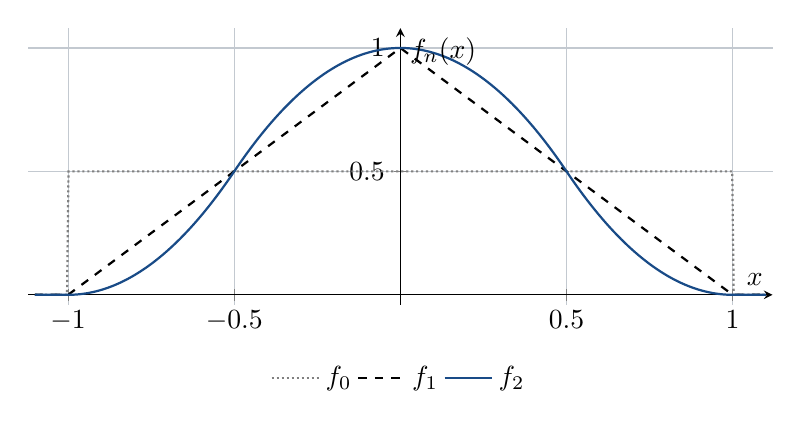
\begin{tikzpicture}
\begin{axis}[
  width=0.91\textwidth,
  height=0.42\textwidth,
  xmin=-1.12,xmax=1.12,
  ymin=-0.04,ymax=1.08,
  axis lines=middle,
  xlabel={$x$},
  ylabel={$f_n(x)$},
  xtick={-1,-0.5,0,0.5,1},
  ytick={0,0.5,1},
  grid=both,
  major grid style={draw=rulegray},
  minor grid style={draw=rulegray!45},
  legend style={at={(0.5,-0.18)},anchor=north,legend columns=3,draw=none},
  samples=501
]
\addplot[thick,gray,densely dotted,domain=-1.1:1.1]
  {abs(x)<1 ? 0.5 : 0};
\addlegendentry{$f_0$}
\addplot[thick,dashed,domain=-1.1:1.1]
  {max(1-abs(x),0)};
\addlegendentry{$f_1$}
\addplot[thick,linkblue,domain=-1.1:1.1]
  {abs(x)<=0.5 ? 1-2*x^2 : (abs(x)<=1 ? 2*(1-abs(x))^2 : 0)};
\addlegendentry{$f_2$}
\end{axis}
\end{tikzpicture}
\caption{The rectangle, the piecewise linear tent, and the quadratic spline.  Later
iterates add one polynomial degree and one smoothness order at each step.}
\label{fig:first-iterates}
\end{figure}

\section{Replacing the last tail: the exact error decomposition}
\label{sec:error-decomposition}

Put
\begin{equation}
 S_n=\sum_{k=1}^{n}2^{-k}U_k,
 \qquad a_n=2^{-n},
 \label{eq:Sn-an}
\end{equation}
and let $p_n$ be the density of $S_n$.  Let $X'$ be an independent copy of the limiting
random variable $X$.  The finite and infinite laws split as
\begin{equation}
 X_n\stackrel d=S_n+a_nU,
 \qquad
 X\stackrel d=S_n+a_nX'.
 \label{eq:tail-replacement}
\end{equation}
If
\begin{equation}
 \rho_a(x)=a^{-1}\Up(x/a)
 \label{eq:scaled-up-density}
\end{equation}
then \eqref{eq:tail-replacement} is exactly
\begin{equation}
 f_n=p_n\conv u_{a_n},
 \qquad
 \Up=p_n\conv\rho_{a_n}.
 \label{eq:finite-infinite-convolution-split}
\end{equation}
The repeated-integration approximation therefore does one very specific thing: it keeps the
first $n$ dyadic uniform coordinates exact and replaces the remaining self-similar tail
$a_nX'$ by a single uniform coordinate $a_nU$.

\subsection{The comparison kernel}

\begin{definition}[Uniform-versus-up Peano kernel]
\label{def:comparison-kernel}
For $t\in\R$, define
\begin{equation}
 K(t)=\E\pos{U-t}-\E\pos{X-t}.
 \label{eq:K-definition}
\end{equation}
\end{definition}

The kernel contains every constant needed for the sharp error theorem.  We first calculate
its basic invariants.

\begin{lemma}[Second and first absolute moments]
\label{lem:up-moments}
The limiting random variable $X$ satisfies
\begin{equation}
 \E X^2=\frac19,
 \qquad
 \E|X|=\frac5{18}.
 \label{eq:X-moments}
\end{equation}
Consequently,
\begin{equation}
 F\left(\frac14\right)=\frac5{72}.
 \label{eq:F-quarter}
\end{equation}
\end{lemma}

\begin{proof}
Independence and centering in \eqref{eq:up-random-series} give
\[
 \E X^2=\frac13\sum_{k=1}^{\infty}4^{-k}=\frac19.
\]
For fixed $x\in[-1,1]$ and $U$ uniform on $[-1,1]$,
\[
 \E\bigl(|x+U|\mid x\bigr)=\frac12\int_{-1}^{1}|x+u|\dd u
 =\frac{1+x^2}{2}.
\]
Using $X\stackrel d=(X'+U)/2$ gives
\[
 \E|X|=\frac12\E|X'+U|
 =\frac14\bigl(1+\E X^2\bigr)=\frac5{18}.
\]
By symmetry, $\E X_+=\frac12\E|X|=5/36$.  On the other hand,
\eqref{eq:X-tail-F} and $F'(y)=2F(2y)$ imply
\[
 \E X_+=\int_0^1F\left(\frac{1-t}{2}\right)\dd t
 =2\int_0^{1/2}F(y)\dd y=2F\left(\frac14\right),
\]
which proves \eqref{eq:F-quarter}.
\end{proof}

\begin{theorem}[Exact kernel data]
\label{thm:kernel-data}
The kernel $K$ is even, continuous, supported in $[-1,1]$, and nonnegative.  For
$0\le t\le1$,
\begin{equation}
 K(t)=\frac{(1-t)^2}{4}-2F\left(\frac{1-t}{4}\right).
 \label{eq:K-explicit}
\end{equation}
Moreover,
\begin{equation}
 \boxed{\displaystyle
 \int_{-1}^{1}K(t)\dd t=\frac19,
 \qquad
 \norm{K}_\infty=K(0)=\frac19,}
 \label{eq:K-mass-and-max}
\end{equation}
while
\begin{equation}
 \norm{K'}_\infty=\frac{13}{72}.
 \label{eq:Kprime-max}
\end{equation}
\end{theorem}

\begin{proof}
Evenness follows from symmetry and the fact that $U$ and $X$ have the same mean.  Both
variables are supported in $[-1,1]$, so $K$ vanishes outside that interval.

For nonnegativity, let $\phi$ be convex.  From the fixed-point identity
$X\stackrel d=(X'+U)/2$ and convexity,
\[
 \E\phi(X)\le\frac12\E\phi(X')+\frac12\E\phi(U).
\]
Since $X'$ has the same law as $X$, this rearranges to
$\E\phi(X)\le\E\phi(U)$.  Thus $X$ is below $U$ in convex order.  Applying this to
$\phi_t(y)=\pos{y-t}$ gives $K(t)\ge0$.

For $0\le t\le1$,
\[
 \E\pos{U-t}=\frac{(1-t)^2}{4}.
\]
Also, by \eqref{eq:X-tail-F},
\begin{align*}
 \E\pos{X-t}
 &=\int_t^1\Prob(X>s)\dd s
 =\int_t^1F\left(\frac{1-s}{2}\right)\dd s\\
 &=2\int_0^{(1-t)/2}F(y)\dd y
 =2F\left(\frac{1-t}{4}\right),
\end{align*}
which proves \eqref{eq:K-explicit}.

The Peano identity proved in \cref{lem:peano-identity} below, applied to
$h(y)=y^2/2$, gives
\[
 \int K(t)\dd t=\frac12\bigl(\E U^2-\E X^2\bigr)
 =\frac12\left(\frac13-\frac19\right)=\frac19.
\]
At the origin, \cref{lem:up-moments} gives
\[
 K(0)=\E U_+-\E X_+=\frac14-\frac5{36}=\frac19.
\]
It remains to see that this is the maximum.  Differentiating
\eqref{eq:K-explicit} gives
\begin{equation}
 K'(t)=F\left(\frac{1-t}{2}\right)-\frac{1-t}{2}.
 \label{eq:Kprime-F}
\end{equation}
On $[0,1/2]$, the Fabius function is convex: $F'(y)=2F(2y)$ is increasing.  Since
$F(0)=0$ and $F(1/2)=1/2$, convexity places its graph below the chord, so
$F(y)\le y$.  Therefore $K'(t)\le0$ for $t\ge0$, and $K(0)$ is the maximum.

Finally, put $y=(1-t)/2$ in \eqref{eq:Kprime-F}.  The magnitude of $K'$ is the maximum of
$y-F(y)$ on $[0,1/2]$.  Its derivative is $1-2F(2y)$, which vanishes exactly at
$y=1/4$ because $F(1/2)=1/2$.  Thus
\[
 \norm{K'}_\infty=\frac14-F\left(\frac14\right)
 =\frac14-\frac5{72}=\frac{13}{72}.
\]
\end{proof}

The equality between the mass and the maximum in \eqref{eq:K-mass-and-max} is the key
numerical coincidence behind the clean final rate.  The mass controls all sufficiently
smooth stages; the maximum controls the borderline stage at which a distributional
box-spline derivative becomes an ordinary continuous error function.

\subsection{Peano identity and the pointwise error formula}

\begin{lemma}[Peano identity]
\label{lem:peano-identity}
Let $h'$ be absolutely continuous on $[-1,1]$.  Then
\begin{equation}
 \E h(U)-\E h(X)=\int_{-1}^{1}K(t)h''(t)\dd t.
 \label{eq:peano-identity}
\end{equation}
\end{lemma}

\begin{proof}
For $y\in[-1,1]$,
\[
 h(y)=h(-1)+h'(-1)(y+1)+\int_{-1}^{1}\pos{y-t}h''(t)\dd t.
\]
Take expectations first with $y=U$ and then with $y=X$.  The constant terms cancel, and
the linear terms cancel because both random variables have mean zero.  Fubini's theorem
then gives \eqref{eq:peano-identity}.
\end{proof}

Apply the lemma with $h(y)=p_n^{(r)}(x-a_ny)$.  Whenever $n\ge r+3$, the needed weak
second derivative is bounded and the result is an ordinary integral.

\begin{proposition}[Exact pointwise error identity]
\label{prop:pointwise-error}
Let $r\ge0$ and $n\ge r+3$.  Then for every $x\in\R$,
\begin{equation}
 f_n^{(r)}(x)-\Up^{(r)}(x)
 =a_n^2\int_{-1}^{1}K(t)
 p_n^{(r+2)}(x-a_nt)\dd t.
 \label{eq:exact-pointwise-error}
\end{equation}
\end{proposition}

\begin{proof}
From \eqref{eq:finite-infinite-convolution-split},
\[
 f_n^{(r)}(x)=\E p_n^{(r)}(x-a_nU),
 \qquad
 \Up^{(r)}(x)=\E p_n^{(r)}(x-a_nX).
\]
Use \cref{lem:peano-identity}; differentiating twice with respect to its argument contributes
the factor $a_n^2$.
\end{proof}

There is also a distributional form that remains valid at the borderline stage.  Define
\begin{equation}
 G_a(x)=aK(x/a).
 \label{eq:Ga-definition}
\end{equation}
Since $K''$ is the difference between the densities of $U$ and $X$ in the distributional
sense,
\begin{equation}
 u_a-\rho_a=\D^2G_a.
 \label{eq:kernel-distribution-identity}
\end{equation}
Consequently,
\begin{equation}
 f_n-\Up=p_n\conv\D^2G_{a_n}.
 \label{eq:error-distribution-convolution}
\end{equation}
This identity will handle the first two smoothness thresholds without any appeal to a
classical second derivative of $p_n$.

\section{Sharp derivative geometry of the partial densities}
\label{sec:partial-density-geometry}

The pointwise identity \eqref{eq:exact-pointwise-error} becomes sharp because the derivatives
of $p_n$ are disjoint signed translates of a single tail density, each having a flat top of
known width and height.

For $m\ge0$, define the dyadic centers
\begin{equation}
 c_{m,j}=-1+\frac{2j+1}{2^m},
 \qquad 0\le j<2^m.
 \label{eq:cmj-definition}
\end{equation}
For $m=0$, this is the singleton $\{0\}$.  At the top piecewise-polynomial derivative
order, derivatives below are understood through their bounded almost-everywhere
representatives; values at the finitely many knots may be chosen arbitrarily between the
adjacent limits and do not affect the $L^\infty$ norm used in this section.

\begin{theorem}[Derivative decomposition and exact plateaux]
\label{thm:partial-derivative-geometry}
Let $0\le m\le n-1$.  Let $q_{m,n}$ be the density of the tail sum
\begin{equation}
 R_{m,n}=\sum_{k=m+1}^{n}2^{-k}U_k.
 \label{eq:Rmn}
\end{equation}
Then, almost everywhere,
\begin{equation}
 p_n^{(m)}(x)=2^{\binom m2}
 \sum_{j=0}^{2^m-1}(-1)^{\wt(j)}q_{m,n}(x-c_{m,j}).
 \label{eq:pnm-decomposition}
\end{equation}
The translated supports in this sum have disjoint interiors.  Moreover,
\begin{equation}
 \norm{p_n^{(m)}}_\infty=2^{\binom{m+1}{2}},
 \label{eq:pnm-norm}
\end{equation}
and on the central interval of each translated tail,
\begin{equation}
 p_n^{(m)}(x)=(-1)^{\wt(j)}2^{\binom{m+1}{2}}
 \quad\text{whenever}\quad |x-c_{m,j}|<2^{-n}.
 \label{eq:pnm-plateau}
\end{equation}
\end{theorem}

\begin{proof}
In the distributional sense,
\begin{equation}
 \D u_{2^{-k}}=2^{k-1}\bigl(\delta_{-2^{-k}}-\delta_{2^{-k}}\bigr).
 \label{eq:uniform-derivative-delta}
\end{equation}
Differentiate the first $m$ factors in
$p_n=u_{2^{-1}}\conv\cdots\conv u_{2^{-n}}$.  The product of the scalar factors is
\[
 \prod_{k=1}^{m}2^{k-1}=2^{\binom m2}.
\]
The $2^m$ signed sums of the locations $\pm2^{-k}$ are precisely the centers
$c_{m,j}$, in increasing order, and the sign is $(-1)^{\wt(j)}$.  Convolution with the
undifferentiated tail gives \eqref{eq:pnm-decomposition}.

Adjacent centers are separated by $2^{1-m}$.  The support radius of $q_{m,n}$ is
\[
 \sum_{k=m+1}^{n}2^{-k}=2^{-m}-2^{-n},
\]
so its support diameter is $2^{1-m}-2^{1-n}$, strictly smaller than the center spacing.
Hence the translated interiors are disjoint.

Scaling shows
\begin{equation}
 q_{m,n}(x)=2^m p_{n-m}(2^mx).
 \label{eq:qmn-scaling}
\end{equation}
The density $p_s$ has supremum one: its first factor $u_{1/2}$ has height one, and
convolution with a probability density cannot increase the supremum.  It actually equals
one on $|x|<2^{-s}$, because the remaining factors have total support radius
$1/2-2^{-s}$.  Thus $q_{m,n}$ has height $2^m$ and is constant at that height on
$|x|<2^{-n}$.  Multiplying by $2^{\binom m2}$ proves
\eqref{eq:pnm-norm} and \eqref{eq:pnm-plateau}.
\end{proof}

At the missing endpoint $m=n$, the same calculation gives a signed Dirac comb:
\begin{equation}
 \D^np_n=2^{\binom n2}
 \sum_{j=0}^{2^n-1}(-1)^{\wt(j)}\delta_{c_{n,j}}.
 \label{eq:pn-top-delta-comb}
\end{equation}
The centers are spaced by $2^{1-n}=2a_n$.

\subsection{A sharp derivative norm for the up-function}

The finite plateau geometry also recovers a useful sharp fact about the limit itself.

\begin{corollary}[Exact derivative peaks of $\Up$]
\label{cor:up-derivative-norm}
For every $m\ge0$,
\begin{equation}
 \boxed{\displaystyle
 \norm{\Up^{(m)}}_\infty=2^{\binom{m+1}{2}}.}
 \label{eq:up-derivative-norm}
\end{equation}
More precisely,
\begin{equation}
 \Up^{(m)}(c_{m,j})=(-1)^{\wt(j)}2^{\binom{m+1}{2}}
 \qquad(0\le j<2^m).
 \label{eq:up-derivative-peaks}
\end{equation}
\end{corollary}

\begin{proof}
Take $n\ge m+1$.  Since $\Up=p_n\conv\rho_{a_n}$,
\[
 \Up^{(m)}(x)=\int p_n^{(m)}(x-y)\rho_{a_n}(y)\dd y.
\]
Convolution with a probability density cannot exceed
$\norm{p_n^{(m)}}_\infty$, giving the upper bound.  At $x=c_{m,j}$, the whole support
$[-a_n,a_n]$ of $\rho_{a_n}$ lies in the constant plateau
\eqref{eq:pnm-plateau}, so the convolution equals the signed plateau height.  This proves
both statements.
\end{proof}

\begin{corollary}[Higher-order flatness at the peak grid]
\label{cor:higher-flatness-grid}
For every $q\ge0$, every $0\le j<2^q$, and every $k>q$,
\begin{equation}
 \Up^{(k)}(c_{q,j})=0.
 \label{eq:higher-flatness-grid}
\end{equation}
\end{corollary}

\begin{proof}
At $q=0$, the only point is $c_{0,0}=0$.  On the right of zero,
$\Up(x)=F(1-x)$, and the smooth bounded Fabius function is constant on $[1,\infty)$;
therefore all positive-order derivatives of $\Up$ vanish at zero.

Let $q\ge1$, put $a=2^{-q}$, and write $\Up=p_q\conv\rho_a$.  For
$\ell=k-q\ge1$,
\[
 \Up^{(k)}=(\D^q p_q)\conv\rho_a^{(\ell)}.
\]
Insert the signed Dirac comb \eqref{eq:pn-top-delta-comb}.  At $x=c_{q,j}$ every
off-diagonal translate is evaluated at distance at least $2a$, outside the support
$[-a,a]$ of $\rho_a$.  The diagonal translate is
$\rho_a^{(\ell)}(0)=a^{-\ell-1}\Up^{(\ell)}(0)=0$ by the first paragraph.
Thus every term vanishes.
\end{proof}

\section{The exact convergence rate}
\label{sec:exact-rate}

We now combine the nonnegative kernel of \cref{sec:error-decomposition} with the exact
plateaux of \cref{sec:partial-density-geometry}.

\subsection{All stages after the first admissible one}

\begin{theorem}[Sharp $L^\infty$ error for every derivative]
\label{thm:sharp-derivative-error}
Let $r\ge0$ and $n\ge r+2$.  Then
\begin{equation}
 \norm{f_n^{(r)}-\Up^{(r)}}_\infty
 =\frac{4^{-n}}{9}\norm{\Up^{(r+2)}}_\infty
 =\frac{2^{\binom{r+3}{2}}}{9\,4^n}.
 \label{eq:sharp-derivative-error}
\end{equation}
At the grid \eqref{eq:error-extremizer-grid}, the signed equality
\eqref{eq:signed-extremizer-error} holds.
\end{theorem}

\begin{proof}
Put $m=r+2$.

First suppose $n\ge m+1$.  From \eqref{eq:exact-pointwise-error}, the nonnegativity and
mass of $K$, and \eqref{eq:pnm-norm},
\begin{align*}
 |f_n^{(r)}(x)-\Up^{(r)}(x)|
 &\le a_n^2\int K(t)\dd t\,\norm{p_n^{(m)}}_\infty\\
 &=4^{-n}\cdot\frac19\cdot2^{\binom{m+1}{2}}.
\end{align*}
At $x=c_{m,j}$, every point $c_{m,j}-a_nt$ with $-1<t<1$ lies in the constant plateau
\eqref{eq:pnm-plateau}.  Hence no inequality remains:
\[
 f_n^{(r)}(c_{m,j})-\Up^{(r)}(c_{m,j})
 =(-1)^{\wt(j)}4^{-n}2^{\binom{m+1}{2}}\int K(t)\dd t.
\]
This proves the result for $n\ge m+1$.

It remains to treat the borderline case $n=m$.  Use
\eqref{eq:error-distribution-convolution} and move all $m=r+2$ derivatives to $p_m$:
\[
 f_m^{(r)}-\Up^{(r)}=(\D^mp_m)\conv G_{a_m}.
\]
By \eqref{eq:pn-top-delta-comb},
\begin{equation}
 f_m^{(r)}(x)-\Up^{(r)}(x)
 =2^{\binom m2}a_m
 \sum_{j=0}^{2^m-1}(-1)^{\wt(j)}
 K\left(\frac{x-c_{m,j}}{a_m}\right).
 \label{eq:borderline-error-kernel-copies}
\end{equation}
The copies of $K$ have support radius $a_m$ and their centers are $2a_m$ apart, so their
interiors are disjoint.  Therefore
\[
 \norm{f_m^{(r)}-\Up^{(r)}}_\infty
 =2^{\binom m2}a_m\norm K_\infty
 =2^{\binom m2-m}\frac19.
\]
Since
$\binom m2-m=\binom{m+1}{2}-2m$, this is exactly the right side of
\eqref{eq:sharp-derivative-error} with $n=m$.  At $x=c_{m,j}$, use $K(0)=1/9$ to obtain
the signed formula.
\end{proof}

The two cases of the proof use different geometric data:
\begin{itemize}
\item for $n\ge r+3$, the error averages a constant extremal plateau and uses
$\int K=1/9$;
\item for $n=r+2$, the error is a disjoint sum of rescaled kernel copies and uses
$\norm K_\infty=1/9$.
\end{itemize}
The equality of those two kernel constants is exactly what makes the same formula valid at
the threshold and beyond it.

\subsection{The first \texorpdfstring{$C^r$}{C-r} spline}

The first iterate with $r$ continuous derivatives is $f_{r+1}$.  Its error has a different
constant, controlled by $K'$ rather than by $K$.

\begin{theorem}[Exceptional first stage]
\label{thm:first-admissible-stage}
For every $r\ge0$,
\begin{equation}
 \norm{f_{r+1}^{(r)}-\Up^{(r)}}_\infty
 =2^{\binom{r+1}{2}}\norm{K'}_\infty
 =\frac{13}{72}2^{\binom{r+1}{2}}.
 \label{eq:first-stage-full}
\end{equation}
The supremum is attained at every point $c_{r+2,k}$, and the signed value is
\eqref{eq:signed-first-stage-error}.
\end{theorem}

\begin{proof}
Set $n=r+1$.  In \eqref{eq:error-distribution-convolution}, the total derivative order is
$r+2=n+1$.  Move $n$ derivatives to $p_n$ and one to $G_{a_n}$.  Since
$G_{a_n}'(x)=K'(x/a_n)$, \eqref{eq:pn-top-delta-comb} gives
\begin{equation}
 f_n^{(r)}(x)-\Up^{(r)}(x)
 =2^{\binom n2}\sum_{j=0}^{2^n-1}(-1)^{\wt(j)}
 K'\left(\frac{x-c_{n,j}}{a_n}\right).
 \label{eq:first-stage-Kprime-copies}
\end{equation}
Again the supports have disjoint interiors, so the supremum is
$2^{\binom n2}\norm{K'}_\infty$.  Substitute $n=r+1$ and
\eqref{eq:Kprime-max}.

For the signed values, \eqref{eq:Kprime-F} gives
$K'(-1/2)=13/72$ and $K'(1/2)=-13/72$.  The two points
$c_{n,j}\mp a_n/2$ are respectively $c_{n+1,2j}$ and $c_{n+1,2j+1}$; using
$\tau_{n+1}(2j)=\tau_n(j)$ and
$\tau_{n+1}(2j+1)=-\tau_n(j)$ in
\eqref{eq:first-stage-Kprime-copies} proves
\eqref{eq:signed-first-stage-error}.
\end{proof}

\subsection{Exact \texorpdfstring{$C^r$}{C-r} convergence}

Because the constants in \eqref{eq:sharp-derivative-error} increase strictly with the
derivative order, the highest derivative controls the max norm \eqref{eq:Cr-norm}.

\begin{corollary}[Exact $C^r$ norm]
\label{cor:exact-Cr-rate}
For every $r\ge0$,
\begin{equation}
 \norm{f_{r+1}-\Up}_{C^r}
 =\frac{13}{72}2^{\binom{r+1}{2}},
 \label{eq:first-Cr-error}
\end{equation}
and for every $n\ge r+2$,
\begin{equation}
 \boxed{\displaystyle
 \norm{f_n-\Up}_{C^r}
 =\frac{2^{\binom{r+3}{2}}}{9\,4^n}.}
 \label{eq:exact-Cr-rate}
\end{equation}
Thus, for every fixed $r$, the tail of the sequence lies in $C^r(\R)$ and converges to
$\Up$ in the $C^r$ norm; the error is exactly geometric from the second admissible stage
onward.  No finite $f_n$ is itself $C^\infty$, so this is deliberately stated as eventual
convergence in every finite smoothness norm rather than literally as convergence of a
sequence inside the Fr\'echet space $C^\infty(\R)$.
\end{corollary}

\begin{proof}
For $n\ge r+2$, the constants in \eqref{eq:sharp-derivative-error} grow strictly with the
derivative order, since the ratio of the order-$(j+1)$ constant to the order-$j$ constant
is $2^{j+3}$.  Hence the $r$th derivative controls the maximum in
\eqref{eq:Cr-norm}.  At the exceptional stage $n=r+1$, the assertion is immediate for
$r=0$.  For $r\ge1$, the largest lower-order error is the order-$(r-1)$ error, and its
ratio to the order-$r$ error in \eqref{eq:first-stage-full} is
\[
 \frac{2^{\binom{r+2}{2}}/(9\,4^{r+1})}
 {(13/72)2^{\binom{r+1}{2}}}
 =\frac{2^{2-r}}{13}<1.
\]
Thus the highest available derivative controls the max norm at the first stage as well.
\end{proof}

For the tent indexing $g_m=f_{m+1}$, this becomes the following direct answer to the
piecewise-linear formulation.

\begin{corollary}[Repeated integration starting from the tent]
\label{cor:tent-indexed-rate}
Let $g_0(x)=\pos{1-|x|}$ and $g_{m+1}=Tg_m$.  For every $r\ge0$,
\begin{equation}
 \norm{g_r-\Up}_{C^r}
 =\frac{13}{72}2^{\binom{r+1}{2}},
 \label{eq:tent-first-Cr}
\end{equation}
and, for every $m\ge r+1$,
\begin{equation}
 \boxed{\displaystyle
 \norm{g_m-\Up}_{C^r}
 =\frac{2^{\binom{r+3}{2}-2}}{9\,4^m}.}
 \label{eq:tent-Cr-rate}
\end{equation}
In particular, \eqref{eq:tent-uniform-rate} holds.
\end{corollary}

\subsection{The uniform errors and exact extremal values}

For $r=0$, the complete startup behavior is
\begin{equation}
 \norm{f_0-\Up}_\infty=\frac12,
 \qquad
 \norm{f_1-\Up}_\infty=\frac{13}{72},
 \qquad
 \norm{f_n-\Up}_\infty=\frac{8}{9\,4^n}\quad(n\ge2).
 \label{eq:all-uniform-errors}
\end{equation}
The value for $f_0$ is immediate from $\Up(0)=1$ and $0\le\Up\le1$.  For $f_1$, put
$y=1-|x|$.  By \eqref{eq:up-F-relation},
\begin{equation}
 f_1(x)-\Up(x)=y-F(y),
 \label{eq:f1-error-F}
\end{equation}
whose absolute maximum is attained at $y=1/4$ and equals
$1/4-F(1/4)=13/72$.

The four extremizers from \eqref{eq:error-extremizer-grid} are
$\pm1/4,\pm3/4$.  Since
\begin{equation}
 \Up(\pm3/4)=F(1/4)=\frac5{72},
 \qquad
 \Up(\pm1/4)=1-F(1/4)=\frac{67}{72},
 \label{eq:up-quarter-values}
\end{equation}
we obtain exact finite-stage values for every $n\ge2$:
\begin{align}
 f_n(\pm3/4)&=\frac5{72}+\frac{8}{9\,4^n},
 \label{eq:fn-threequarter}\\
 f_n(\pm1/4)&=\frac{67}{72}-\frac{8}{9\,4^n}.
 \label{eq:fn-onequarter}
\end{align}
The first few are shown in \cref{tab:exact-errors}.

\begin{table}[htbp]
\centering
\caption{Sharp uniform errors and two extremal values.}
\label{tab:exact-errors}
\begin{tabular}{c@{\qquad}c@{\qquad}c@{\qquad}c}
\toprule
$n$&$\norm{f_n-\Up}_\infty$&$f_n(3/4)$&$f_n(1/4)$\\
\midrule
$0$&$1/2$&--&--\\
$1$&$13/72$&$1/4$&$3/4$\\
$2$&$1/18$&$1/8$&$7/8$\\
$3$&$1/72$&$1/12$&$11/12$\\
$4$&$1/288$&$7/96$&$89/96$\\
$5$&$1/1152$&$9/128$&$119/128$\\
$6$&$1/4608$&$107/1536$&$1429/1536$\\
\bottomrule
\end{tabular}
\end{table}

\section{The asymptotic error profile}
\label{sec:asymptotic-profile}

The exact norm formula gives the rate, but the Peano identity also identifies the whole
limiting error shape.

\begin{theorem}[Uniform leading profile]
\label{thm:leading-profile}
For every fixed $r\ge0$,
\begin{equation}
 4^n\bigl(f_n^{(r)}-\Up^{(r)}\bigr)
 \longrightarrow \frac19\Up^{(r+2)}
 \qquad\text{uniformly on }\R.
 \label{eq:leading-profile}
\end{equation}
\end{theorem}

\begin{proof}
Put $m=r+2$.  From \eqref{eq:exact-pointwise-error},
\[
 4^n\bigl(f_n^{(r)}(x)-\Up^{(r)}(x)\bigr)
 =\int K(t)p_n^{(m)}(x-a_nt)\dd t.
\]
For fixed $m$, $p_n^{(m)}\to\Up^{(m)}$ uniformly.  One direct estimate follows from
$\Up=p_n\conv\rho_{a_n}$ and the mean-value theorem:
\[
 \norm{p_n^{(m)}-\Up^{(m)}}_\infty
 \le a_n\E|X|\,\norm{p_n^{(m+1)}}_\infty,
\]
for all sufficiently large $n$.  The same derivative bound shows that replacing
$p_n^{(m)}(x-a_nt)$ by $p_n^{(m)}(x)$ costs $O(a_n)$ uniformly.  Finally use
$\int K=1/9$.
\end{proof}

Combining \eqref{eq:leading-profile} with \eqref{eq:up-derivative-norm} predicts the sharp
constant in \eqref{eq:sharp-derivative-error}.  The exact theorem says more: the norm of the
leading profile is already the exact norm of the full error for every $n\ge r+2$.

\subsection{A full even-derivative expansion}

The Fourier product provides an all-orders refinement.  Put
\begin{equation}
 \Phi(z)=\prod_{k=1}^{\infty}\sinc(z/2^k),
 \qquad
 A(z)=\frac{\sinc z}{\Phi(z)}.
 \label{eq:A-ratio}
\end{equation}
The quotient is analytic near the origin (indeed on $|z|<2\pi$) and meromorphic
globally.  Wherever $\Phi(2^{-n}t)\ne0$ one has
\begin{equation}
 \mathscr F f_n(t)=\mathscr F\Up(t)A(2^{-n}t),
 \label{eq:fourier-ratio}
\end{equation}
and at the exceptional frequencies the product on the right is interpreted by its
continuous finite-product extension.  Only the Taylor germ at zero is used below.  It is
convenient to encode that germ by
\begin{equation}
 B(w)=A(\iu w)
 =\frac{\sinh w/w}{\displaystyle\prod_{k=1}^{\infty}
 \frac{\sinh(w/2^k)}{w/2^k}}
 =\sum_{m=0}^{\infty}\beta_mw^{2m}.
 \label{eq:B-generating}
\end{equation}
The first coefficients are
\begin{equation}
 \beta_0=1,
 \qquad \beta_1=\frac19,
 \qquad \beta_2=\frac{2}{2025},
 \qquad \beta_3=-\frac1{2679075},
 \qquad \beta_4=\frac{58}{10247461875}.
 \label{eq:beta-first}
\end{equation}

\begin{proposition}[All-orders $C^r$ expansion]
\label{prop:all-orders-expansion}
For fixed integers $r\ge0$ and $M\ge1$,
\begin{equation}
 f_n^{(r)}
 =\sum_{m=0}^{M-1}\beta_m4^{-mn}\Up^{(r+2m)}
 +O_{r,M}(4^{-Mn})
 \label{eq:all-orders-expansion}
\end{equation}
uniformly on $\R$ as $n\to\infty$.
\end{proposition}

\begin{proof}
Choose $R$ with $1<R<2\pi$ and put $a=2^{-n}$.  On $|z|\le R$, Taylor's theorem gives
\begin{equation}
 A(z)=\sum_{m=0}^{M-1}\beta_m(-1)^m z^{2m}+O_{M,R}(|z|^{2M}).
 \label{eq:A-Taylor-remainder}
\end{equation}
On the low-frequency region $|t|\le R/a$, multiply this by
$(\iu t)^r\mathscr F\Up(t)$.  Since $\mathscr F\Up$ is a Schwartz function, the
$L^1$ norm of the resulting remainder is at most
\[
 C_{r,M,R}a^{2M}\int_{\R}|t|^{r+2M}|\mathscr F\Up(t)|\dd t
 =O_{r,M}(a^{2M}).
\]
The sign in \eqref{eq:A-Taylor-remainder} is exactly the sign in
$(\iu t)^{2m}=(-1)^mt^{2m}$, so Fourier inversion produces the displayed derivatives of
$\Up$.

It remains to control $|t|>R/a$.  From \eqref{eq:finite-fourier-product} and
$|\sinc y|\le\min(1,|y|^{-1})$, for $|t|\ge R2^n$,
\begin{equation}
 |\mathscr F f_n(t)|
 \le 2^{n(n+1)/2+n}|t|^{-(n+1)}.
 \label{eq:finite-product-high-frequency}
\end{equation}
Hence, for fixed $r$ and large $n$,
\[
 \int_{|t|>R2^n}|t|^r|\mathscr F f_n(t)|\dd t
 \le C_r R^{r-n}2^{-n^2/2+(r+3/2)n},
\]
which is smaller than $a^{2M}$ for all sufficiently large $n$.  The high-frequency tails
of the finitely many $\Up^{(r+2m)}$ terms are also $O_{r,M}(a^{2M})$, again because
$\mathscr F\Up$ is Schwartz.  Fourier inversion now proves the uniform remainder in
\eqref{eq:all-orders-expansion}.
\end{proof}

For explicit coefficient generation, write
\begin{equation}
 \log B(w)=\sum_{m=1}^{\infty}\lambda_mw^{2m}.
 \label{eq:lambda-log}
\end{equation}
With the standard Bernoulli numbers $B_{2m}$,
\begin{equation}
 \lambda_m=
 \frac{2^{2m-1}B_{2m}}{m(2m)!}
 \frac{4^m-2}{4^m-1}.
 \label{eq:lambda-formula}
\end{equation}
Indeed,
\[
 \log\frac{\sinh w}{w}
 =\sum_{m\ge1}\frac{2^{2m-1}B_{2m}}{m(2m)!}w^{2m},
 \qquad
 \sum_{k\ge1}4^{-mk}=\frac1{4^m-1};
\]
subtracting the logarithms of the denominator factors in \eqref{eq:B-generating} gives
\eqref{eq:lambda-formula}.  The coefficients $\beta_m$ are then obtained recursively from
\begin{equation}
 \beta_0=1,
 \qquad
 \beta_m=\frac1m\sum_{j=1}^{m}j\lambda_j\beta_{m-j}.
 \label{eq:beta-recurrence}
\end{equation}
Thus the first terms of \eqref{eq:all-orders-expansion} are
\begin{equation}
 f_n^{(r)}=\Up^{(r)}
 +\frac{\Up^{(r+2)}}{9\,4^n}
 +\frac{2\Up^{(r+4)}}{2025\,16^n}
 -\frac{\Up^{(r+6)}}{2679075\,64^n}
 +O_r(256^{-n}).
 \label{eq:first-asymptotic-terms}
\end{equation}
At the extremal grid \eqref{eq:error-extremizer-grid}, all higher derivative terms vanish
by \cref{cor:higher-flatness-grid}; there the leading term is not merely asymptotic but
exactly equal to the full error, as \eqref{eq:signed-extremizer-error} states.

\section{Exact computation and numerical use}
\label{sec:computation}

\subsection{A direct exact-arithmetic evaluator}

Formula \eqref{eq:exact-iterate-intro} immediately gives an exact rational evaluator at
rational arguments.  The following compact Python implementation uses arbitrary-precision
fractions.  It is intended as executable notation rather than as the fastest large-$n$
algorithm.

\begin{lstlisting}[style=reportcode,language=Python,caption={Exact evaluation of the finite iterates.},label={lst:exact-evaluator}]
from fractions import Fraction
from math import factorial


def tau(n: int, j: int) -> int:
    if j < 0 or j >= (1 << n):
        return 0
    return -1 if (j.bit_count() & 1) else 1


def positive_power(x: Fraction, n: int) -> Fraction:
    return x**n if x > 0 else Fraction(0)


def f(n: int, x: Fraction) -> Fraction:
    x = Fraction(x)
    if n == 0:
        return Fraction(1, 2) if abs(x) < 1 else Fraction(0)

    coefficient = Fraction(
        1 << (n * (n + 1) // 2 - 1), factorial(n)
    )
    mesh = Fraction(1, 1 << (n - 1))

    return coefficient * sum(
        (tau(n, j) - tau(n, j - 1))
        * positive_power(x + 1 - j * mesh, n)
        for j in range((1 << n) + 1)
    )
\end{lstlisting}

Only indices satisfying $j<2^{n-1}(x+1)$ contribute, so the loop may be truncated at the
active cell.  Derivatives are obtained by replacing $n!$ with $(n-r)!$ and the power $n$
with $n-r$, as in \eqref{eq:finite-spline-derivatives}.

\subsection{Conditioning and stable evaluation}

The truncated-power formula is exact but can exhibit severe cancellation at large $n$:
individual terms are much larger than their sum.  Three alternatives are preferable in
floating-point work.

\begin{enumerate}[label=\textup{(\roman*)}]
\item Use the convolution description \eqref{eq:fn-box-convolution} and propagate a
piecewise-polynomial representation from one level to the next.
\item Use a B-spline/de Boor representation on the dyadic knot sequence rather than the
truncated-power basis.
\item In Fourier space, evaluate the finite sinc product \eqref{eq:finite-fourier-product}
and invert it with a quadrature adapted to a compactly supported smooth target.
\end{enumerate}

For certified approximation of $\Up$, the sharp error gives an immediate stopping rule.  To
obtain uniform error at most $\varepsilon$ from the tent-indexed sequence, it is necessary
and sufficient that
\begin{equation}
 m\ge
 \ceil{\frac12\log_2\left(\frac{2}{9\varepsilon}\right)}
 \qquad(m\ge1).
 \label{eq:stopping-rule}
\end{equation}
For a fixed derivative order $r$, replace the numerator $2/9$ by
$2^{\binom{r+3}{2}-2}/9$ and also require $m\ge r+1$.

\section{How this fits the existing ProveIt development}
\label{sec:formalization-roadmap}

The present approximation is closely related to, but not identical with, two families
already developed in the repository.

\begin{itemize}
\item The finite convolution and polynomial machinery in
\nolinkurl{FabiusFunction/EarlyApproximants.lean} provides reusable measure-theoretic and
coefficient infrastructure.
\item The Thue--Morse spline machinery in
\nolinkurl{FabiusFunction/FabiusUniformSpline.lean} already contains many of the finite-power
sum and block-translation lemmas needed to identify the top derivative pattern.
\item The centered finite-CDF spline in the main article approximates the bounded Fabius
function.  The sequence here approximates the up-density itself and has a different tail
replacement and a different sharp rate.
\end{itemize}

A natural formalization could be organized as follows.

\begin{enumerate}[label=\textup{(\arabic*)}]
\item Define the probability operator $T$ and prove
$Th(x)=\int_{2x-1}^{2x+1}h$ for supported integrable $h$.
\item Define $X_n$ recursively and prove the finite random-sum identity
\eqref{eq:Xn-random-sum}; derive \eqref{eq:fn-box-convolution} at the level of measures.
\item Introduce the nonuniform box spline and prove the general inclusion--exclusion lemma
\eqref{eq:general-box-spline}.
\item Reuse the finite Thue--Morse product to prove
\eqref{eq:first-difference-generating}, then obtain the exact iterate and derivative formulas.
\item Define $K$ by \eqref{eq:K-definition}.  Prove convex domination with the one-line
Jensen argument, then formalize its mass, maximum, and derivative maximum.
\item Prove the derivative decomposition \eqref{eq:pnm-decomposition}, support separation,
and the exact plateaux.
\item Combine the Peano identity with the plateau lemma, splitting the proof into the
ordinary case $n\ge r+3$ and the distributional threshold $n=r+2$.
\end{enumerate}

The analytic core of the sharp theorem is therefore modest.  The technically delicate
parts for Lean are likely to be bookkeeping for weak derivatives of interval densities and
the transfer between measure convolution and classical derivatives.  One can avoid most
of that friction by proving the borderline formulas directly from finite signed Dirac
combs and using ordinary absolutely continuous derivatives only after the threshold.

\section{Conclusions}
\label{sec:conclusion}

The repeated-integration construction has three mutually reinforcing exact descriptions:

\begin{enumerate}[label=\textup{(\roman*)}]
\item an averaging recursion $X\mapsto(X+U)/2$;
\item a convolution of dyadically scaled uniform densities;
\item a dyadic polynomial spline whose top derivative is a Thue--Morse word.
\end{enumerate}

These descriptions identify the limit as Rvachev's up-function and reduce the finite-stage
closed form to a single first-difference Thue--Morse sum.  More unexpectedly, the same
probabilistic representation yields a completely sharp convergence theorem.  The finite
stage and the limit differ only in the last scaled tail: a uniform variable replaces an
up-distributed variable.  Their mass and mean agree, so the error starts at second order in
$2^{-n}$.  The comparison kernel quantifies this replacement exactly, while the partial
box spline supplies disjoint extremal plateaux.  The outcome is the exact identity
\[
 \norm{f_n^{(r)}-\Up^{(r)}}_\infty
 =\frac{2^{\binom{r+3}{2}}}{9\,4^n}
 \qquad(n\ge r+2),
\]
not just an upper bound or an asymptotic equivalent.

In the most literal piecewise-linear formulation, starting from the tent and integrating
again and again, the answer is especially crisp: after the initial tent, the uniform error
is exactly $2/(9\,4^m)$.  Every additional integration divides the worst-case error by four,
and the points at which that error is attained are fixed dyadic points rather than moving
with the iteration.

\begin{thebibliography}{99}

\bibitem{mse-question}
kram1032,
\emph{Recursive Integration over Piecewise Polynomials: Closed form?},
Mathematics Stack Exchange, question 240687, 19 November 2012,
\url{https://math.stackexchange.com/questions/240687/recursive-integration-over-piecewise-polynomials-closed-form}.

\bibitem{mse-answer}
Nathan Grigg,
\emph{Answer to ``Recursive Integration over Piecewise Polynomials: Closed form?''},
Mathematics Stack Exchange, 22 November 2012,
\url{https://math.stackexchange.com/a/240805}.

\bibitem{arias1982}
Juan Arias de Reyna,
\emph{An infinitely differentiable function with compact support: Definition and
properties},
English translation, arXiv:1702.05442, 2017; original Spanish version in
\emph{Revista de la Real Academia de Ciencias Exactas, Físicas y Naturales de Madrid}
\textbf{76} (1982), 21--38.

\bibitem{arias2018}
Juan Arias de Reyna,
\emph{Arithmetic of the Fabius function},
arXiv:1702.06487; \emph{Integers} \textbf{18} (2018), A51.

\bibitem{fabius1966}
Jaap Fabius,
\emph{A probabilistic example of a nowhere analytic $C^\infty$-function},
\emph{Zeitschrift für Wahrscheinlichkeitstheorie und Verwandte Gebiete}
\textbf{5} (1966), 173--174.

\bibitem{jessen-wintner1935}
Børge Jessen and Aurel Wintner,
\emph{Distribution functions and the Riemann zeta function},
\emph{Transactions of the American Mathematical Society}
\textbf{38} (1935), 48--88.

\bibitem{proveit}
Vladimir Reshetnikov,
\emph{ProveIt: Analysis/FabiusFunction},
\url{https://github.com/VladimirReshetnikov/ProveIt/tree/main/Analysis/FabiusFunction},
repository snapshot consulted 25 August 2026.

\end{thebibliography}

\end{document}
